\begin{enumerate}[label=\thesubsection.\arabic*., ref=\thesubsection.\theenumi]
\numberwithin{equation}{enumi}
%%%%%%%%%%%%%%%%%%%% Q5 %%%%%%%%%%%%%%%%%%%%
\setcounter{enumi}{4}
\item In Figure-1, if tangents $PA$ and $PB$ from an external point $\vec{P}$ to a circle with centre $\vec{O}$, are inclined to each other at an angle of $80^{\circ}$, then $\angle AOB$ is equal to
\begin{enumerate}
\item $100^{\circ}$
\item $60^{\circ}$
\item $80^{\circ}$
\item $50^{\circ}$
\end{enumerate}
\hfill (CBSE Class 10)
 
\solution Since $PA$ and $PB$ are tangents, from \eqref{eq:c10-tangent},
\begin{align}
\brak{\vec{A}-\vec{O}}^{\top}\brak{\vec{P}-\vec{A}} = 0,\quad
\brak{\vec{B}-\vec{O}}^{\top}\brak{\vec{P}-\vec{B}} = 0
\end{align}
so $\angle OAP = \angle OBP = 90^{\circ}$. In the quadrilateral $OAPB$, from \eqref{eq:c10-quad},
\begin{align}
\angle AOB = 360^{\circ} - 90^{\circ} - 90^{\circ} - 80^{\circ} = 100^{\circ}
\end{align}
This is verified with \eqref{eq:c10-angle} in the code, which gives
\begin{align}
\cos\theta = \frac{\brak{\vec{A}-\vec{O}}^{\top}\brak{\vec{B}-\vec{O}}}{\norm{\vec{A}-\vec{O}}\norm{\vec{B}-\vec{O}}}
= \cos 100^{\circ}
\end{align}
Hence, the correct option is (a).
 
\begin{figure}[H]
\centering
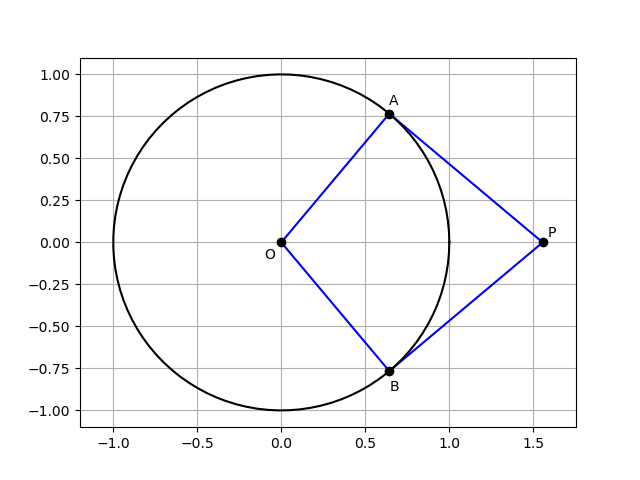
\includegraphics[width=0.6\columnwidth]{figs/q5_tangents.png}
\caption{Tangents $PA$ and $PB$ with $\angle APB = 80^{\circ}$}
\label{fig:c10-q5}
\end{figure}
 
\begin{center}
\fbox{\parbox{0.9\columnwidth}{\centering codes/q5.py}}
\end{center}
 
%%%%%%%%%%%%%%%%%%%% Q6 %%%%%%%%%%%%%%%%%%%%
\setcounter{enumi}{5}
\item The mean and median of a distribution are $10$ and $14$ respectively. The value of mode is
\begin{enumerate}
\item $6$
\item $22$
\item $2$
\item $20$
\end{enumerate}
\hfill (CBSE Class 10)
 
\solution From \eqref{eq:c10-empirical},
\begin{align}
\text{mode} = 3\,\text{median} - 2\,\text{mean} = 3\brak{14} - 2\brak{10} = 22
\end{align}
Hence, the correct option is (b).
 
\begin{center}
\fbox{\parbox{0.9\columnwidth}{\centering codes/q6.c}}
\end{center}
 
%%%%%%%%%%%%%%%%%%%% Q8 %%%%%%%%%%%%%%%%%%%%
\setcounter{enumi}{7}
\item The value(s) of $k$ for which the quadratic equation $3x^2-kx+3=0$ has equal roots, is (are)
\begin{enumerate}
\item $6$
\item $-6$
\item $\pm 6$
\item $9$
\end{enumerate}
\textbf{OR}\\
The discriminant of the quadratic equation $3\sqrt{3}x^2+10x+\sqrt{3}=0$ is
\begin{enumerate}
\item $\pm 8$
\item $8$
\item $100-4\sqrt{3}$
\item $64$
\end{enumerate}
\hfill (CBSE Class 10)
 
\solution Here $a=3$, $b=-k$, $c=3$. The roots are equal when $D=0$, so from \eqref{eq:c10-disc},
\begin{align}
k^2-4\brak{3}\brak{3} = 0
\implies k^2 = 36
\implies k = \pm 6
\end{align}
Hence, the correct option is (c).
 
\textbf{OR} Here $a=3\sqrt{3}$, $b=10$, $c=\sqrt{3}$. From \eqref{eq:c10-disc},
\begin{align}
D = 10^2-4\brak{3\sqrt{3}}\brak{\sqrt{3}} = 100-36 = 64
\end{align}
Hence, the correct option is (d).
 
\begin{center}
\fbox{\parbox{0.9\columnwidth}{\centering codes/q8.c}}
\end{center}
 
%%%%%%%%%%%%%%%%%%%% Q9 %%%%%%%%%%%%%%%%%%%%
\setcounter{enumi}{8}
\item Two dice are thrown simultaneously. The probability that the sum of two numbers appearing on the top of the dice is less than $12$, is
\begin{enumerate}
\item $\frac{1}{36}$
\item $\frac{35}{36}$
\item $0$
\item $1$
\end{enumerate}
\hfill (CBSE Class 10)
 
\solution Let $X$ and $Y$ be the numbers on the two dice and $S=X+Y$. The pmf of one die is $p[n]=\frac{1}{6}$ for $n=1,\dots,6$. From \eqref{eq:c10-ztrans},
\begin{align}
H(z) = \frac{1}{6}\brak{z^{-1}+z^{-2}+z^{-3}+z^{-4}+z^{-5}+z^{-6}}
\end{align}
Since the dice are independent, from \eqref{eq:c10-conv},
\begin{align}
H_S(z) = H(z)^2
= \frac{1}{36}\brak{z^{-2}+2z^{-3}+3z^{-4}+\dots+6z^{-7}+\dots+2z^{-11}+z^{-12}}
\end{align}
The coefficient of $z^{-12}$ is $\Pr\brak{S=12}=\frac{1}{36}$. Therefore
\begin{align}
\Pr\brak{S<12} = 1-\Pr\brak{S=12} = 1-\frac{1}{36} = \frac{35}{36}
\end{align}
Hence, the correct option is (b).
 
\begin{figure}[H]
\centering
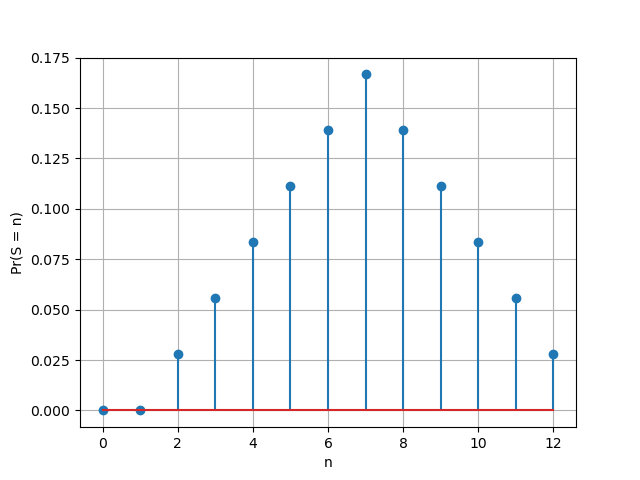
\includegraphics[width=0.7\columnwidth]{figs/q9_dice.png}
\caption{Distribution of the sum of two dice}
\label{fig:c10-q9}
\end{figure}
 
\begin{center}
\fbox{\parbox{0.9\columnwidth}{\centering codes/q9.py}}
\end{center}
 
%%%%%%%%%%%%%%%%%%%% Q10 %%%%%%%%%%%%%%%%%%%%
\setcounter{enumi}{9}
\item A frustum of a right circular cone which is of height $8$ cm with radii of its circular ends as $10$ cm and $4$ cm, has its slant height equal to
\begin{enumerate}
\item $14$ cm
\item $28$ cm
\item $10$ cm
\item $\sqrt{260}$ cm
\end{enumerate}
\hfill (CBSE Class 10)
 
\solution Here $h=8$, $R=10$, $r=4$. From \eqref{eq:c10-frustum},
\begin{align}
l = \sqrt{8^2+\brak{10-4}^2} = \sqrt{64+36} = \sqrt{100} = 10
\end{align}
Hence, the correct option is (c).
 
\begin{center}
\fbox{\parbox{0.9\columnwidth}{\centering codes/q10.c}}
\end{center}
 
%%%%%%%%%%%%%%%%%%%% Q13 %%%%%%%%%%%%%%%%%%%%
\setcounter{enumi}{12}
\item A line intersecting a circle at two points is called a \underline{\hspace{2cm}}.\\
\textbf{OR}\\
The tangents drawn at the ends of a diameter of a circle are \underline{\hspace{2cm}}.
\hfill (CBSE Class 10)
 
\solution A line meeting a circle at two points is a {\em secant}. For the circle $x^2+y^2=1$ and the line $y=0.5$, the distance $d=0.5<r=1$, so the line meets the circle at two points.
 
\textbf{OR} Let $\vec{A}=\myvec{1\\0}$ and $\vec{B}=\myvec{-1\\0}$ be the ends of a diameter. The tangent directions are perpendicular to $\vec{A}-\vec{O}$ and $\vec{B}-\vec{O}$,
\begin{align}
\vec{m}_1 = \myvec{0\\1},\quad \vec{m}_2 = \myvec{0\\-1}
\end{align}
From \eqref{eq:c10-parallel},
\begin{align}
\det\myvec{\vec{m}_1 & \vec{m}_2} = \begin{vmatrix}0&0\\1&-1\end{vmatrix} = 0
\end{align}
Hence, the answers are {\em secant} and {\em parallel}.
 
\begin{center}
\fbox{\parbox{0.9\columnwidth}{\centering codes/q13.c}}
\end{center}
 
%%%%%%%%%%%%%%%%%%%% Q14 %%%%%%%%%%%%%%%%%%%%
\setcounter{enumi}{13}
\item The value of $m$ which makes the points $\brak{0,0}$, $\brak{2m,-4}$ and $\brak{3,6}$ collinear, is \underline{\hspace{2cm}}.
\hfill (CBSE Class 10)
 
\solution Let $\vec{A}=\myvec{0\\0}$, $\vec{B}=\myvec{2m\\-4}$, $\vec{C}=\myvec{3\\6}$. From \eqref{eq:c10-collinear},
\begin{align}
\begin{vmatrix}2m&3\\-4&6\end{vmatrix} = 12m+12 = 0
\implies m = -1
\end{align}
Hence, $m=-1$.
 
\begin{center}
\fbox{\parbox{0.9\columnwidth}{\centering codes/q14.c}}
\end{center}
 
%%%%%%%%%%%%%%%%%%%% Q15 %%%%%%%%%%%%%%%%%%%%
\setcounter{enumi}{14}
\item If $\alpha,\beta$ are zeroes of the polynomial $2x^2-5x-4$, then $\frac{1}{\alpha}+\frac{1}{\beta}=$ \underline{\hspace{2cm}}.
\hfill (CBSE Class 10)
 
\solution From \eqref{eq:c10-zeroes}, $\alpha+\beta=\frac{5}{2}$ and $\alpha\beta=-2$. Then
\begin{align}
\frac{1}{\alpha}+\frac{1}{\beta} = \frac{\alpha+\beta}{\alpha\beta}
= \frac{5/2}{-2} = -\frac{5}{4}
\end{align}
Hence, the answer is $-\frac{5}{4}$.
 
\begin{center}
\fbox{\parbox{0.9\columnwidth}{\centering codes/q15.c}}
\end{center}
 
%%%%%%%%%%%%%%%%%%%% Q16 %%%%%%%%%%%%%%%%%%%%
\setcounter{enumi}{15}
\item The capacity of a cylindrical glass tumbler is $125.6\ \text{cm}^3$. If the radius of the glass tumbler is $2$ cm, then find its height. (Use $\pi=3.14$)
\hfill (CBSE Class 10)
 
\solution From \eqref{eq:c10-cyl},
\begin{align}
h = \frac{V}{\pi r^2} = \frac{125.6}{3.14\times 4} = 10\ \text{cm}
\end{align}
Hence, the height is $10$ cm.
 
\begin{center}
\fbox{\parbox{0.9\columnwidth}{\centering codes/q16.c}}
\end{center}
 
%%%%%%%%%%%%%%%%%%%% Q17 %%%%%%%%%%%%%%%%%%%%
\setcounter{enumi}{16}
\item A circle has its centre at $\brak{4,4}$. If one end of a diameter is $\brak{4,0}$, then find the coordinates of the other end.
\hfill (CBSE Class 10)
 
\solution Let $\vec{O}=\myvec{4\\4}$ and $\vec{A}=\myvec{4\\0}$. The centre is the midpoint of the diameter, so from \eqref{eq:c10-mid},
\begin{align}
\vec{B} = 2\myvec{4\\4}-\myvec{4\\0} = \myvec{4\\8}
\end{align}
Hence, the other end is $\brak{4,8}$.
 
\begin{center}
\fbox{\parbox{0.9\columnwidth}{\centering codes/q17.c}}
\end{center}
 
%%%%%%%%%%%%%%%%%%%% Q18 %%%%%%%%%%%%%%%%%%%%
\setcounter{enumi}{17}
\item If two positive integers $p$ and $q$ can be expressed as $p=ab^3$ and $q=a^2b$; $a$ and $b$ being prime numbers, then find LCM of $\brak{p,q}$.
\hfill (CBSE Class 10)
 
\solution The LCM takes the highest power of each prime from \eqref{eq:c10-lcm},
\begin{align}
\text{LCM}\brak{p,q} = a^2b^3
\end{align}
For $a=2$, $b=3$: $p=54$, $q=12$, HCF $=6$ and
\begin{align}
\text{LCM} = \frac{54\times 12}{6} = 108 = 2^2\times 3^3
\end{align}
Hence, $\text{LCM}\brak{p,q}=a^2b^3$.
 
\begin{center}
\fbox{\parbox{0.9\columnwidth}{\centering codes/q18.c}}
\end{center}
 
%%%%%%%%%%%%%%%%%%%% Q19 %%%%%%%%%%%%%%%%%%%%
\setcounter{enumi}{18}
\item It is given that $\triangle ABC\sim\triangle PQR$ with $\frac{BC}{QR}=\frac{1}{3}$, then find the value of $\frac{\text{ar}\brak{PRQ}}{\text{ar}\brak{ACB}}$.
\hfill (CBSE Class 10)
 
\solution From \eqref{eq:c10-simarea},
\begin{align}
\frac{\text{ar}\brak{ABC}}{\text{ar}\brak{PQR}} = \brak{\frac{1}{3}}^2 = \frac{1}{9}
\end{align}
Since $\text{ar}\brak{PRQ}=\text{ar}\brak{PQR}$ and $\text{ar}\brak{ACB}=\text{ar}\brak{ABC}$,
\begin{align}
\frac{\text{ar}\brak{PRQ}}{\text{ar}\brak{ACB}} = 9
\end{align}
Hence, the answer is $9$.
 
\begin{center}
\fbox{\parbox{0.9\columnwidth}{\centering codes/q19.c}}
\end{center}
 
%%%%%%%%%%%%%%%%%%%% Q20 %%%%%%%%%%%%%%%%%%%%
\setcounter{enumi}{19}
\item In Figure-2, a tower stands vertically on the ground. From a point on the ground, which is $80$ m away from the foot of the tower, the angle of elevation of the tower is found to be $30^{\circ}$. Find the height of the tower.
\hfill (CBSE Class 10)
 
\solution Let $\vec{B}$ be the foot of the tower, $\vec{A}$ the point on the ground and $\vec{C}$ the top,
\begin{align}
\vec{B} = \myvec{0\\0},\quad \vec{A} = \myvec{80\\0},\quad \vec{C} = \myvec{0\\h}
\end{align}
From \eqref{eq:c10-tan},
\begin{align}
\tan 30^{\circ} = \frac{BC}{AB} = \frac{h}{80}
\implies h = \frac{80}{\sqrt{3}} = \frac{80\sqrt{3}}{3} \approx 46.19\ \text{m}
\end{align}
Hence, the height of the tower is $\frac{80\sqrt{3}}{3}$ m.
 
\begin{figure}[H]
\centering
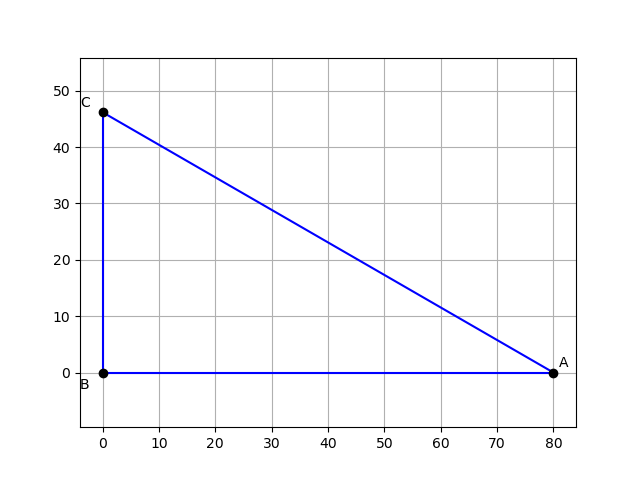
\includegraphics[width=0.6\columnwidth]{figs/q20_tower.png}
\caption{Tower $BC$ with angle of elevation $30^{\circ}$ at $A$}
\label{fig:c10-q20}
\end{figure}
 
\begin{center}
\fbox{\parbox{0.9\columnwidth}{\centering codes/q20.py}}
\end{center}
 
%%%%%%%%%%%%%%%%%%%% Q21 %%%%%%%%%%%%%%%%%%%%
\setcounter{enumi}{20}
\item Show that any positive odd integer is of the form $4q+1$ or $4q+3$ for some integer $q$.
\hfill (CBSE Class 10)
 
\solution Let $n$ be a positive integer. From \eqref{eq:c10-euclid} with $d=4$,
\begin{align}
n = 4q+r, \qquad r\in\cbrak{0,1,2,3}
\end{align}
For $r=0$ and $r=2$, $n=4q$ and $n=4q+2$ are even. So if $n$ is odd, $r=1$ or $r=3$,
\begin{align}
n = 4q+1 \quad \text{or} \quad n = 4q+3
\end{align}
The code checks that $n \bmod 4\in\cbrak{1,3}$ for every odd $n<100$.
 
\begin{center}
\fbox{\parbox{0.9\columnwidth}{\centering codes/q21.c}}
\end{center}
 
%%%%%%%%%%%%%%%%%%%% Q22 %%%%%%%%%%%%%%%%%%%%
\setcounter{enumi}{21}
\item In Figure-3, $PQ\parallel BC$, $PQ=3$ cm, $BC=9$ cm and $AC=7.5$ cm. Find the length of $AQ$.
\hfill (CBSE Class 10)
 
\solution Since $PQ\parallel BC$, from \eqref{eq:c10-thales},
\begin{align}
k = \frac{PQ}{BC} = \frac{3}{9} = \frac{1}{3}
\end{align}
Then
\begin{align}
AQ = k\,AC = \frac{1}{3}\brak{7.5} = 2.5\ \text{cm}
\end{align}
In the code, $\vec{Q}=\vec{A}+k\brak{\vec{C}-\vec{A}}$ gives $\norm{\vec{Q}-\vec{A}}=2.5$. Hence, $AQ=2.5$ cm.
 
\begin{figure}[H]
\centering
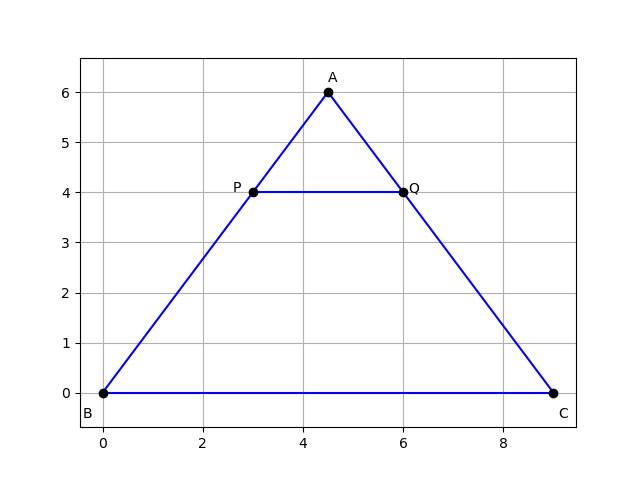
\includegraphics[width=0.6\columnwidth]{figs/q22_triangle.png}
\caption{$PQ\parallel BC$ in $\triangle ABC$}
\label{fig:c10-q22}
\end{figure}
 
\begin{center}
\fbox{\parbox{0.9\columnwidth}{\centering codes/q22.py}}
\end{center}
 
%%%%%%%%%%%%%%%%%%%% Q23 %%%%%%%%%%%%%%%%%%%%
\setcounter{enumi}{22}
\item Solve $9x^2-6a^2x+a^4-b^4=0$ using quadratic formula.
\hfill (CBSE Class 10)
 
\solution Here $A=9$, $B=-6a^2$, $C=a^4-b^4$. The discriminant is
\begin{align}
B^2-4AC = 36a^4-36\brak{a^4-b^4} = 36b^4
\end{align}
From \eqref{eq:c10-quadform},
\begin{align}
x = \frac{6a^2\pm 6b^2}{18} = \frac{a^2\pm b^2}{3}
\end{align}
For $a=2$, $b=1$ the roots are $\frac{5}{3}$ and $1$, as the code shows. Hence, $x=\frac{a^2+b^2}{3}$ or $x=\frac{a^2-b^2}{3}$.
 
\begin{center}
\fbox{\parbox{0.9\columnwidth}{\centering codes/q23.c}}
\end{center}
 
%%%%%%%%%%%%%%%%%%%% Q24 %%%%%%%%%%%%%%%%%%%%
\setcounter{enumi}{23}
\item A jar contains $18$ marbles. Some are red and others are yellow. If a marble is drawn at random from the jar, the probability that it is red is $\frac{2}{3}$. Find the number of yellow marbles in the jar.\\
\textbf{OR}\\
A die is thrown twice. What is the probability that
\begin{enumerate}
\item $5$ will come up at least once, and
\item $5$ will not come up either time?
\end{enumerate}
\hfill (CBSE Class 10)
 
\solution From \eqref{eq:c10-prob}, the number of red marbles is
\begin{align}
18\times\frac{2}{3} = 12
\end{align}
so the number of yellow marbles is $18-12=6$.
 
\textbf{OR} The die has $6\times 6=36$ outcomes. A $5$ does not come up either time in $5\times 5=25$ outcomes, so from \eqref{eq:c10-prob},
\begin{align}
\Pr\brak{\text{no }5} = \frac{25}{36},\qquad
\Pr\brak{\text{at least one }5} = 1-\frac{25}{36} = \frac{11}{36}
\end{align}
Hence, the answers are $6$ yellow marbles, and $\frac{11}{36}$ and $\frac{25}{36}$.
 
\begin{figure}[H]
\centering
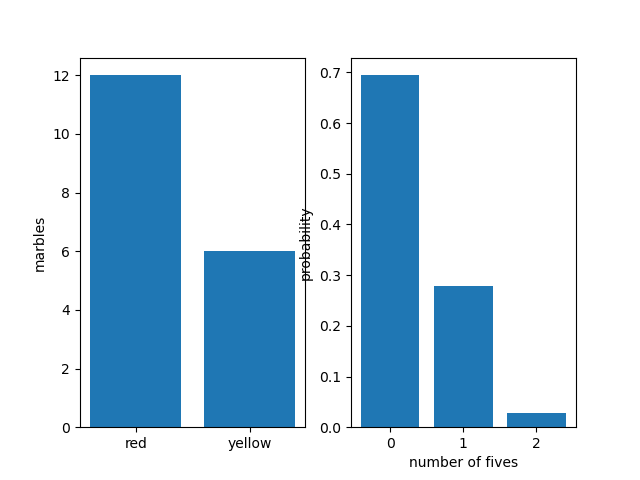
\includegraphics[width=0.8\columnwidth]{figs/q24_probability.png}
\caption{Marbles in the jar and the number of fives in two throws}
\label{fig:c10-q24}
\end{figure}
 
\begin{center}
\fbox{\parbox{0.9\columnwidth}{\centering codes/q24.py}}
\end{center}
 
%%%%%%%%%%%%%%%%%%%% Q26 %%%%%%%%%%%%%%%%%%%%
\setcounter{enumi}{25}
\item Find mode of the following distribution:
\begin{center}
\begin{tabular}{|l|c|c|c|c|c|c|}
\hline
Class & 25--30 & 30--35 & 35--40 & 40--45 & 45--50 & 50--55 \\
\hline
Frequency & 20 & 36 & 53 & 40 & 28 & 14 \\
\hline
\end{tabular}
\end{center}
\hfill (CBSE Class 10)
 
\solution The highest frequency is $53$, so the modal class is $35$--$40$. Here $l=35$, $h=5$, $f_1=53$, $f_0=36$, $f_2=40$. From \eqref{eq:c10-mode},
\begin{align}
\text{mode} = 35+\frac{53-36}{2\brak{53}-36-40}\times 5
= 35+\frac{17}{30}\times 5 = 35+\frac{17}{6} = \frac{227}{6}\approx 37.83
\end{align}
Hence, the mode is $37.83$.
 
\begin{center}
\fbox{\parbox{0.9\columnwidth}{\centering codes/q26.c}}
\end{center}
 
%%%%%%%%%%%%%%%%%%%% Q28 (OR) %%%%%%%%%%%%%%%%%%%%
\setcounter{enumi}{27}
\item If the points $\vec{A}\brak{2,0}$, $\vec{B}\brak{6,1}$ and $\vec{C}\brak{p,q}$ form a triangle of area $12$ sq. units (positive only) and $2p+q=10$, then find the values of $p$ and $q$.
\hfill (CBSE Class 10)
 
\solution The vertices are
\begin{align}
\vec{A}=\myvec{2\\0},\quad \vec{B}=\myvec{6\\1},\quad \vec{C}=\myvec{p\\q}
\end{align}
From \eqref{eq:c10-area}, taking the area as $+12$,
\begin{align}
\frac{1}{2}\begin{vmatrix}4&p-2\\1&q\end{vmatrix} = \frac{1}{2}\brak{4q-p+2} = 12
\implies -p+4q = 22
\end{align}
Together with $2p+q=10$, the system in matrix form is
\begin{align}
\myvec{-1&4\\2&1}\myvec{p\\q} = \myvec{22\\10}
\end{align}
The determinant of the matrix is $-1-8=-9$, so
\begin{align}
\myvec{p\\q} = \frac{1}{-9}\myvec{1&-4\\-2&-1}\myvec{22\\10}
= \frac{1}{-9}\myvec{-18\\-54} = \myvec{2\\6}
\end{align}
Hence, $p=2$ and $q=6$.
 
\begin{figure}[H]
\centering
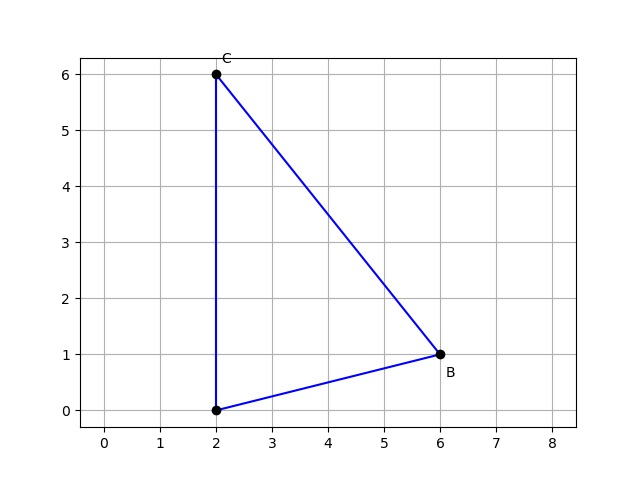
\includegraphics[width=0.6\columnwidth]{figs/q28_triangle.png}
\caption{Triangle $ABC$ with $\vec{C}=\brak{2,6}$}
\label{fig:c10-q28}
\end{figure}
 
\begin{center}
\fbox{\parbox{0.9\columnwidth}{\centering codes/q28.py}}
\end{center}
 
%%%%%%%%%%%%%%%%%%%% Q30 (OR) %%%%%%%%%%%%%%%%%%%%
\setcounter{enumi}{29}
\item Solve the following equations for $x$ and $y$ using cross-multiplication method:
\begin{align}
\brak{ax-by}+\brak{a+4b} = 0,\qquad \brak{bx+ay}+\brak{b-4a} = 0
\end{align}
\hfill (CBSE Class 10)
 
\solution In matrix form,
\begin{align}
\myvec{a&-b\\b&a}\myvec{x\\y} = \myvec{-\brak{a+4b}\\4a-b}
\end{align}
The determinant is $a^2+b^2\ne 0$. From \eqref{eq:c10-linsys},
\begin{align}
\myvec{x\\y} = \frac{1}{a^2+b^2}\myvec{a&b\\-b&a}\myvec{-a-4b\\4a-b}
= \frac{1}{a^2+b^2}\myvec{-a^2-b^2\\4a^2+4b^2} = \myvec{-1\\4}
\end{align}
Hence, $x=-1$ and $y=4$.
 
\begin{figure}[H]
\centering
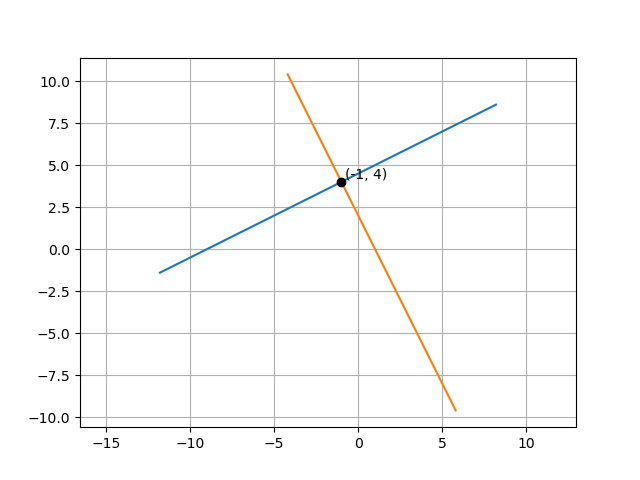
\includegraphics[width=0.6\columnwidth]{figs/q30_lines.png}
\caption{The two lines meet at $\brak{-1,4}$ (plotted for $a=1$, $b=2$)}
\label{fig:c10-q30}
\end{figure}
 
\begin{center}
\fbox{\parbox{0.9\columnwidth}{\centering codes/q30.py}}
\end{center}
 
%%%%%%%%%%%%%%%%%%%% Q31 %%%%%%%%%%%%%%%%%%%%
\setcounter{enumi}{30}
\item Draw a circle of radius $2.5$ cm. Take a point $P$ outside the circle at a distance of $7$ cm from the centre. Then construct a pair of tangents to the circle from point $P$.
\hfill (CBSE Class 10)
 
\solution Take $\vec{O}=\myvec{0\\0}$, $\vec{P}=\myvec{7\\0}$ and $r=2.5$. From \eqref{eq:c10-tangpts}, a tangent point $\vec{A}=\myvec{x_1\\x_2}$ satisfies
\begin{align}
\vec{A}^{\top}\vec{A} = r^2,\qquad \vec{A}^{\top}\brak{\vec{A}-\vec{P}} = 0
\implies \vec{A}^{\top}\vec{P} = r^2
\end{align}
So $7x_1=6.25$ and
\begin{align}
x_1 = \frac{25}{28},\qquad x_2 = \pm\sqrt{6.25-x_1^2} \approx \pm 2.34
\end{align}
The tangent points are $\vec{A}=\myvec{0.89\\2.34}$ and $\vec{B}=\myvec{0.89\\-2.34}$. The tangent length is
\begin{align}
\norm{\vec{P}-\vec{A}} = \sqrt{7^2-2.5^2} = \sqrt{42.75}\approx 6.54\ \text{cm}
\end{align}
Joining $\vec{P}$ to $\vec{A}$ and $\vec{B}$ gives the pair of tangents.
 
\begin{figure}[H]
\centering
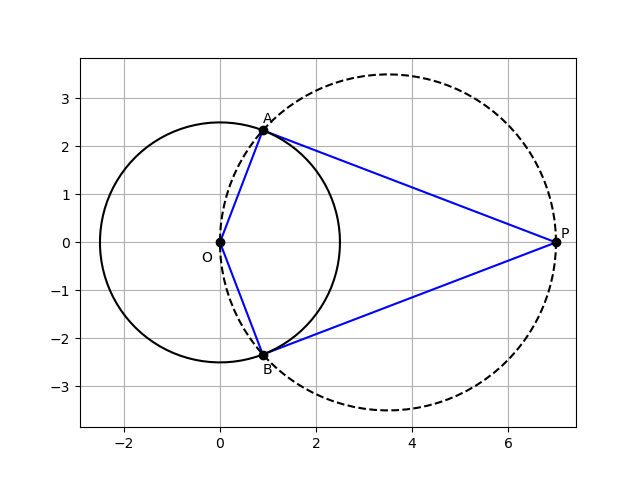
\includegraphics[width=0.7\columnwidth]{figs/q31_tangents.png}
\caption{Tangents $PA$ and $PB$, with the circle on $OP$ as diameter dashed}
\label{fig:c10-q31}
\end{figure}
 
\begin{center}
\fbox{\parbox{0.9\columnwidth}{\centering codes/q31.py}}
\end{center}
 
%%%%%%%%%%%%%%%%%%%% Q32 %%%%%%%%%%%%%%%%%%%%
\setcounter{enumi}{31}
\item A mint moulds four types of copper coins $A,B,C$ and $D$ whose diameters vary from $0.5$ cm to $5$ cm. The first coin $A$ has a diameter of $0.7$ cm. The second coin $B$ has double the diameter of coin $A$ and from then onwards the diameters increase by $50\%$. Thickness of each coin is $0.25$ cm.
\begin{enumerate}
\item Fill in the diameters of the coins required in the table.
\item Complete the table of area of one face and volume. [Use $\pi=\frac{22}{7}$]
\end{enumerate}
\hfill (CBSE Class 10)
 
\solution (i) The diameter of $B$ is $2\times 0.7=1.4$ cm. Then $C$ is $1.5\times 1.4=2.1$ cm and $D$ is $1.5\times 2.1=3.15$ cm.
 
\begin{center}
\begin{tabular}{|c|c|}
\hline
Type of Coin & Diameter (in cm) \\
\hline
A & 0.7 \\
\hline
B & 1.4 \\
\hline
\end{tabular}
\end{center}
 
(ii) From \eqref{eq:c10-coin}, for coin $B$,
\begin{align}
\text{area} = \frac{22}{7}\brak{0.7}^2 = 1.54\ \text{cm}^2,\qquad
\text{volume} = 1.54\times 0.25 = 0.385\ \text{cm}^3
\end{align}
 
\begin{center}
\begin{tabular}{|c|c|c|}
\hline
Type of Coin & Area (in cm$^2$) of one face & Volume (in cm$^3$) \\
\hline
A & 0.385 & 0.09625 \\
\hline
B & 1.54 & 0.385 \\
\hline
\end{tabular}
\end{center}
 
\begin{center}
\fbox{\parbox{0.9\columnwidth}{\centering codes/q32.c}}
\end{center}
 
%%%%%%%%%%%%%%%%%%%% Q35 %%%%%%%%%%%%%%%%%%%%
\setcounter{enumi}{34}
\item Sides $AB$ and $AC$ and median $AD$ of $\triangle ABC$ are respectively proportional to sides $PQ$ and $PR$ and median $PM$ of $\triangle PQR$. Show that $\triangle ABC\sim\triangle PQR$.\\
\textbf{OR}\\
In Figure-4, $BN$ and $CM$ are medians of a $\triangle ABC$ right-angled at $A$. Prove that $4\brak{BN^2+CM^2}=5BC^2$.
\hfill (CBSE Class 10)
 
\solution {\bf Given:}
\begin{align}
\frac{AB}{PQ} = \frac{AC}{PR} = \frac{AD}{PM}
\end{align}
{\bf Construction:} Extend $AD$ to $E$ such that $DE=AD$ and join $BE$, $CE$. Extend $PM$ to $F$ such that $MF=PM$ and join $QF$, $RF$.
 
{\bf Proof:} In the quadrilateral $ABEC$, $D$ is the midpoint of both $BC$ and $AE$ (from \eqref{eq:c10-median}), so the diagonals bisect each other and $ABEC$ is a parallelogram. Hence
\begin{align}
BE = AC,\qquad CE = AB
\end{align}
Similarly $PQFR$ is a parallelogram, so $QF=PR$ and $RF=PQ$. From the given condition,
\begin{align}
\frac{AB}{PQ} = \frac{BE}{QF} = \frac{AE}{PF}
\end{align}
because $\frac{BE}{QF}=\frac{AC}{PR}$ and $\frac{AE}{PF}=\frac{2AD}{2PM}=\frac{AD}{PM}$. By SSS from \eqref{eq:c10-sim},
\begin{align}
\triangle ABE\sim\triangle PQF \implies \angle BAE = \angle QPF
\end{align}
In the same way,
\begin{align}
\frac{AC}{PR} = \frac{CE}{RF} = \frac{AE}{PF}
\implies \triangle ACE\sim\triangle PRF \implies \angle CAE = \angle RPF
\end{align}
Adding the two angle equalities,
\begin{align}
\angle BAC = \angle QPR
\end{align}
Now $\frac{AB}{PQ}=\frac{AC}{PR}$ and $\angle A=\angle P$, so by SAS from \eqref{eq:c10-sim},
\begin{align}
\triangle ABC\sim\triangle PQR
\end{align}
The code checks the three ratios $\frac{AB}{PQ}$, $\frac{AC}{PR}$, $\frac{AD}{PM}$ for a sample pair of triangles.
 
\textbf{OR} Take $\vec{A}=\myvec{0\\0}$, $\vec{B}=\myvec{x\\0}$, $\vec{C}=\myvec{0\\y}$. From \eqref{eq:c10-median} the midpoints are
\begin{align}
\vec{M} = \myvec{x/2\\0},\qquad \vec{N} = \myvec{0\\y/2}
\end{align}
Then
\begin{align}
BN^2 &= \norm{\vec{N}-\vec{B}}^2 = x^2+\frac{y^2}{4}
\\
CM^2 &= \norm{\vec{M}-\vec{C}}^2 = \frac{x^2}{4}+y^2
\end{align}
Adding and using \eqref{eq:c10-pyth},
\begin{align}
BN^2+CM^2 = \frac{5}{4}\brak{x^2+y^2} = \frac{5}{4}BC^2
\implies 4\brak{BN^2+CM^2} = 5BC^2
\end{align}
For $x=8$, $y=4$, the code gives $4\brak{68+32}=400=5\times 80$. Hence proved.
 
\begin{figure}[H]
\centering
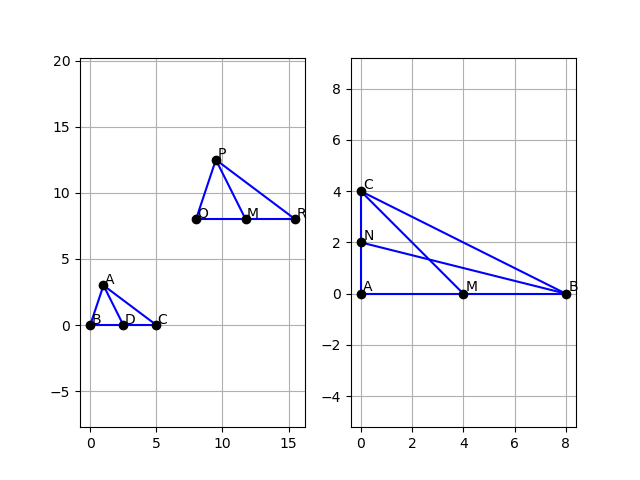
\includegraphics[width=\columnwidth]{figs/q35_medians.png}
\caption{Left: $\triangle ABC$ and $\triangle PQR$ with medians. Right: Figure-4}
\label{fig:c10-q35}
\end{figure}
 
\begin{center}
\fbox{\parbox{0.9\columnwidth}{\centering codes/q35.py}}
\end{center}
 
%%%%%%%%%%%%%%%%%%%% Q36 %%%%%%%%%%%%%%%%%%%%
\setcounter{enumi}{35}
\item The angles of depression of the top and bottom of a tower as seen from the top of a $60\sqrt{3}$ m high cliff are $45^{\circ}$ and $60^{\circ}$ respectively. Find the height of the tower. (Use $\sqrt{3}=1.73$)
\hfill (CBSE Class 10)
 
\solution Let $H=60\sqrt{3}$ be the height of the cliff, $d$ the distance between the cliff and the tower, and $h$ the height of the tower. From \eqref{eq:c10-tan4560}, for the bottom of the tower,
\begin{align}
\tan 60^{\circ} = \frac{H}{d} \implies d = \frac{60\sqrt{3}}{\sqrt{3}} = 60\ \text{m}
\end{align}
For the top of the tower,
\begin{align}
\tan 45^{\circ} = \frac{H-h}{d} = 1 \implies h = H-d = 60\sqrt{3}-60 = 60\brak{\sqrt{3}-1}
\end{align}
With $\sqrt{3}=1.73$,
\begin{align}
h = 60\times 0.73 = 43.8\ \text{m}
\end{align}
Hence, the height of the tower is $43.8$ m.
 
\begin{center}
\fbox{\parbox{0.9\columnwidth}{\centering codes/q36.c}}
\end{center}
 
%%%%%%%%%%%%%%%%%%%% Q37 %%%%%%%%%%%%%%%%%%%%
\setcounter{enumi}{36}
\item A well of diameter $3$ m is dug $14$ m deep. The earth taken out of it has been spread evenly all around it in the shape of a circular ring of width $4$ m to form a platform. Find the height of the platform. (Take $\pi=\frac{22}{7}$)\\
\textbf{OR}\\
In Figure-5, a solid toy is in the form of a hemisphere surmounted by a right circular cone. The height of the cone is $2$ cm and the diameter of the base is $4$ cm. Determine the volume of the toy. (Take $\pi=3.14$)
\hfill (CBSE Class 10)
 
\solution The well is a cylinder with $r=1.5$ m and depth $14$ m. From \eqref{eq:c10-cyl},
\begin{align}
V = \frac{22}{7}\brak{1.5}^2\brak{14} = 99\ \text{m}^3
\end{align}
The ring has inner radius $1.5$ m and outer radius $1.5+4=5.5$ m. From \eqref{eq:c10-vol},
\begin{align}
\frac{22}{7}\brak{5.5^2-1.5^2}H = 99
\implies \frac{22}{7}\brak{28}H = 99
\implies H = \frac{99}{88} = 1.125\ \text{m}
\end{align}
Hence, the height of the platform is $1.125$ m.
 
\textbf{OR} The cone and the hemisphere have $r=2$ cm and the cone has $h=2$ cm. From \eqref{eq:c10-vol},
\begin{align}
V = \frac{1}{3}\pi r^2 h+\frac{2}{3}\pi r^3
= 3.14\brak{\frac{8}{3}+\frac{16}{3}} = 3.14\times 8 = 25.12\ \text{cm}^3
\end{align}
Hence, the volume of the toy is $25.12$ cm$^3$.
 
\begin{center}
\fbox{\parbox{0.9\columnwidth}{\centering codes/q37.c}}
\end{center}
 
%%%%%%%%%%%%%%%%%%%% Q38 %%%%%%%%%%%%%%%%%%%%
\setcounter{enumi}{37}
\item $A$ and $B$ jointly finish a piece of work in $15$ days. When they work separately, $A$ takes $16$ days less than the number of days taken by $B$ to finish the same piece of work. Find the number of days taken by $B$ to finish the work.
\hfill (CBSE Class 10)
 
\solution Let $B$ take $x$ days, so $A$ takes $x-16$ days. From \eqref{eq:c10-work},
\begin{align}
\frac{1}{x}+\frac{1}{x-16} = \frac{1}{15}
\implies 15\brak{2x-16} = x\brak{x-16}
\implies x^2-46x+240 = 0
\end{align}
From \eqref{eq:c10-quadform},
\begin{align}
x = \frac{46\pm\sqrt{2116-960}}{2} = \frac{46\pm 34}{2} = 40 \ \text{or}\ 6
\end{align}
For $x=6$, $A$ would take $6-16<0$ days, which is not possible. Hence, $B$ takes $40$ days.
 
\begin{center}
\fbox{\parbox{0.9\columnwidth}{\centering codes/q38.c}}
\end{center}
 
%%%%%%%%%%%%%%%%%%%% Q39 %%%%%%%%%%%%%%%%%%%%
\setcounter{enumi}{38}
\item If the polynomial $f\brak{x}=3x^4-9x^3+x^2+15x+k$ is completely divisible by $3x^2-5$, then find the value of $k$. Using the quotient, so obtained, find two zeroes of the polynomial.\\
\textbf{OR}\\
Find all the zeroes of the polynomial $x^4-8x^3+23x^2-28x+12$ if two of its zeroes are $2$ and $3$.
\hfill (CBSE Class 10)
 
\solution Dividing $f\brak{x}$ by $3x^2-5$ from \eqref{eq:c10-poly},
\begin{align}
3x^4-9x^3+x^2+15x+k = \brak{3x^2-5}\brak{x^2-3x+2}+\brak{k+10}
\end{align}
Since the division is complete, the remainder is zero,
\begin{align}
k+10 = 0 \implies k = -10
\end{align}
The quotient is $x^2-3x+2=\brak{x-1}\brak{x-2}$, so two zeroes of $f\brak{x}$ are $1$ and $2$. With $f\brak{x}=x^2-3x+2$, \eqref{eq:c10-newton} reads
\begin{align}
x_{n+1} = x_n-\frac{x_n^2-3x_n+2}{2x_n-3}
\end{align}
For $x_0=0$, $x_1=\frac{2}{3}$ and the iterates converge to $1$. For $x_0=3$, $x_1=\frac{7}{3}$ and the iterates converge to $2$, as the code shows. Hence, $k=-10$ and the zeroes are $1$ and $2$.
 
\textbf{OR} Since $2$ and $3$ are zeroes, $\brak{x-2}\brak{x-3}=x^2-5x+6$ divides the polynomial. From \eqref{eq:c10-poly},
\begin{align}
x^4-8x^3+23x^2-28x+12 = \brak{x^2-5x+6}\brak{x^2-3x+2}
\end{align}
The quotient $x^2-3x+2=\brak{x-1}\brak{x-2}$ gives the other zeroes. Newton--Raphson from $x_0=0$, $1.5$ and $4$ converges to $1$, $2$ and $3$ respectively. Hence, all the zeroes are $1,\ 2,\ 2,\ 3$.
 
\begin{center}
\fbox{\parbox{0.9\columnwidth}{\centering codes/q39.py}}
\end{center}
 
%%%%%%%%%%%%%%%%%%%% Q40 %%%%%%%%%%%%%%%%%%%%
\setcounter{enumi}{39}
\item Draw `less than' ogive for the following distribution and hence find its median.
\begin{center}
\begin{tabular}{|c|c|}
\hline
Class & Frequency \\
\hline
20--30 & 10 \\
\hline
30--40 & 8 \\
\hline
40--50 & 12 \\
\hline
50--60 & 24 \\
\hline
60--70 & 6 \\
\hline
70--80 & 25 \\
\hline
80--90 & 15 \\
\hline
\end{tabular}
\end{center}
\hfill (CBSE Class 10)
 
\solution The points of the `less than' ogive are the upper class limits with their cumulative frequencies,
\begin{center}
\begin{tabular}{|c|c|c|c|c|c|c|c|}
\hline
Upper limit & 30 & 40 & 50 & 60 & 70 & 80 & 90 \\
\hline
$cf$ & 10 & 18 & 30 & 54 & 60 & 85 & 100 \\
\hline
\end{tabular}
\end{center}
Plotting these points and joining them gives the ogive. Here $N=100$, so $\frac{N}{2}=50$. The point of the ogive with $y=50$ lies between
\begin{align}
\vec{P}_1 = \myvec{50\\30},\qquad \vec{P}_2 = \myvec{60\\54}
\end{align}
From \eqref{eq:c10-ogive}, the $y$-coordinate gives
\begin{align}
30+\lambda\brak{54-30} = 50 \implies \lambda = \frac{20}{24} = \frac{5}{6}
\end{align}
and the $x$-coordinate, which is the median, is
\begin{align}
x = 50+\frac{5}{6}\brak{60-50} = 50+\frac{25}{3} = \frac{175}{3}\approx 58.33
\end{align}
This agrees with \eqref{eq:c10-gmedian} for the median class $50$--$60$, where $l=50$, $cf=30$, $f=24$, $h=10$,
\begin{align}
\text{median} = 50+\frac{50-30}{24}\times 10 \approx 58.33
\end{align}
Hence, the median is $58.33$.
 
\begin{center}
\fbox{\parbox{0.9\columnwidth}{\centering codes/q40.c}}
\end{center}
 
\end{enumerate}
 
